% image size
\documentclass[20pt]{extarticle}
\usepackage[papersize={1200px,675px},margin=60px]{geometry} % 16:9, e.g. for Twitter or Mastodon

\usepackage[english]{babel}
\usepackage{microtype}

% Colours
% https://latexcolor.com/
\usepackage{xcolor}
\definecolor{aliceblue}{rgb}{0.94, 0.97, 1.0}
\definecolor{eggshell}{rgb}{0.94, 0.92, 0.84}

% Fonts
\usepackage{fontspec}
\usepackage{unicode-math}
\setmainfont{TeX Gyre Bonum}
\setmathfont{TeX Gyre Bonum Math}

\usepackage{tikz}

\begin{document}
    \pagenumbering{gobble}
    \pagecolor{aliceblue}
    \huge
    
    \noindent{\Huge\textbf{Nodes}}
    
    \noindent Two players play on a line of \(n\) nodes, taking turns to draw their symbol in one node. The winner is the first player to draw their symbol in \(\left\lceil \frac{n}{2} \right\rceil\) adjacent nodes. \vspace{3ex}
    
    \centering\normalsize\begin{tikzpicture}[scale=2,every node/.style={scale=2}]
        \node[circle,fill=eggshell,draw,line width=0.5ex,inner sep=3ex] (n0) at (0,0) {};
        \node[circle,fill=eggshell,draw,line width=0.5ex,inner sep=3ex] (n1) at (5,0) {};
        \node[scale=1.5] (dots) at (10,0) {\Huge \(\ldots\)};
        \node[circle,fill=eggshell,draw,line width=0.5ex,inner sep=3ex] (n2) at (15,0) {};
        \draw[-,line width=0.7ex] (n0) -- (n1);
        \draw[-,line width=0.7ex] (n1) -- (dots);
        \draw[-,line width=0.7ex] (dots) -- (n2);
        
    \end{tikzpicture}
    
\end{document}